\subsection{10 PRINT CHR\$(205.5+RND(1)); : GOTO 10}

Все примеры здесь для .COM-файлов под MS-DOS.
%FIXME1 -> about .COM files

\myindex{MS-DOS}
В [Nick Montfort et al, \emph{10 PRINT CHR\$(205.5+RND(1)); : GOTO 10}, (The MIT Press:2012)]
\footnote{\AlsoAvailableAs \url{http://trope-tank.mit.edu/10_PRINT_121114.pdf}}
можно прочитать об одном из простейших генераторов случайных лабиринтов.
Он просто бесконечно и случайно печатает символ слэша или обратный слэш, выдавая в итоге что-то вроде:

\begin{figure}[H]
\centering
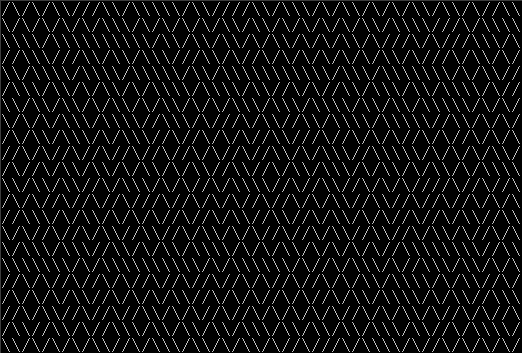
\includegraphics[width=0.8\textwidth]{examples/demos/10print/10print.png}
\end{figure}

Здесь несколько известных реализаций для 16-битного x86.

\subsubsection{Версия 42-х байт от Trixter}

\newcommand{\FNURLTRIXTER}{\footnote{\url{http://trixter.oldskool.org/2012/12/17/maze-generation-in-thirteen-bytes/}}}

Листинг взят с его сайта\FNURLTRIXTER, но комментарии --- автора.

\lstinputlisting[style=customasmx86]{examples/demos/10print/10print_42_RU.lst}

\myindex{Intel!8253}
Псевдослучайное число на самом деле это время, прошедшее со старта системы, получаемое из чипа таймера 8253, 
это значение
увеличивается на единицу 18.2 раза в секунду.

Записывая ноль в порт \TT{43h}, 
мы имеем ввиду что команда это \q{выбрать счетчик 0}, 
"counter latch", 
"двоичный счетчик" (а не значение \ac{BCD}).

\myindex{x86!\Instructions!POPF}
Прерывания снова разрешаются при помощи инструкции \TT{POPF}, которая
также возвращает флаг \TT{IF}.

\myindex{x86!\Instructions!IN}
Инструкцию \TT{IN} нельзя использовать с другими регистрами кроме \TT{AL}, поэтому здесь перетасовка.

\subsubsection{Моя попытка укоротить версию Trixter: 27 байт}

Мы можем сказать, что мы используем таймер не для того чтобы получить точное время, но псевдослучайное число,
так что мы можем не тратить время (и код) на запрещение прерываний.
Еще можно сказать, что так как мы берем бит из младшей 8-битной части, то мы можем считывать только её.

Немного укоротим код и выходит 27 байт:

\lstinputlisting[style=customasmx86]{examples/demos/10print/10print_27_RU.lst}

\subsubsection{Использование случайного мусора в памяти как источника случайных чисел}

Так как это MS-DOS, защиты памяти здесь нет вовсе, так что мы можем читать с какого
угодно адреса.
\myindex{x86!\Instructions!LODSB}
И даже более того: простая инструкция \TT{LODSB} 
будет читать байт по адресу \TT{DS:SI}, но это не проблема
если правильные значения не установлены в регистры, пусть она читает 1) случайные байты; 2) из случайного
места в памяти!

Так что на странице Trixter-а\FNURLTRIXTER 
можно найти предложение использовать \TT{LODSB} без всякой инициализации.

\myindex{x86!\Instructions!SCASB}
Есть также предложение использовать инструкцию \TT{SCASB} 
вместо, потому что она выставляет флаги в соответствии с прочитанным значением.

Еще одна идея насчет минимизации кода --- это использовать прерывание DOS
 \TT{INT 29h} которое просто печатает символ на экране
из регистра \TT{AL}.

Это то что сделал Peter Ferrie
\footnote{\url{http://pferrie.host22.com/misc/10print.htm}}:

\lstinputlisting[caption=Peter Ferrie: 10 байт,style=customasmx86]{examples/demos/10print/ferrie_10_RU.lst}

Так что можно избавиться и от условных переходов.
\ac{ASCII}-код обратного слэша (\q{\textbackslash{}}) 
это \TT{0x5C} и \TT{0x2F} для слэша (\q{/}).

Так что нам нужно конвертировать один (псевдослучайный) бит из флага \TT{CF} в значение \TT{0x5C} или \TT{0x2F}.

Это делается легко: применяя операцию \q{И} ко всем битам в \TT{AL} (где все 8 бит либо выставлены, либо сброшены) с \TT{0x2D} мы имеем просто 0 или \TT{0x2D}.

Прибавляя значение \TT{0x2F} к этому значению, мы получаем \TT{0x5C} или \TT{0x2F}.
И просто выводим это на экран.

\subsubsection{\Conclusion{}}

\myindex{DOSBox}
Также стоит отметить, что результат может быть разным в эмуляторе DOSBox, \gls{Windows NT} и даже MS-DOS, 
из-за разных условий:
чип таймера может эмулироваться по-разному, изначальные значения регистров также могут быть разными.
